\documentclass[12pt]{article}
\usepackage[utf8]{inputenc}
\usepackage{graphicx}
\usepackage[a4paper,width=150mm,top=25mm,bottom=25mm]{geometry}

\title{{IBM Data Science Capstone Report}
}



\author{Leslie Chiu}

\begin{document}

\maketitle


\begin{abstract}
This report use data from Foursqaure to help a business owner make the decision about where to open the restaurant
\end{abstract}

\section{Introduction}
Mr. Sammon is a Korean immigrant and he is good at cooking. He wants to establish his own business by openning a Korean style restaurant in Toronto. However, he doesn't know the business environment in Toronto and people's lifestyles, thus has been struggling deciding where to open his business. We would like to conduct some analysis in this report and offer him some advice regarding this question.

\section{Data}
We use three different datasets, first two are what we have been using in the last week's project, which includes lists of postal codes of Canada and the geographical information. The third data set we will use in addition is the lists of venues obtained from Foursquare. We will combine these datasets and use them to see in which neighborhood the competition is not too harsh so that Mr. Sammon has a chance to make a profit.

\section{Methodology}
I first do some data visualization. I restrict my attention to downtown Toronto and plot all the neighborhoods in the following map to visually show their distributions.\\
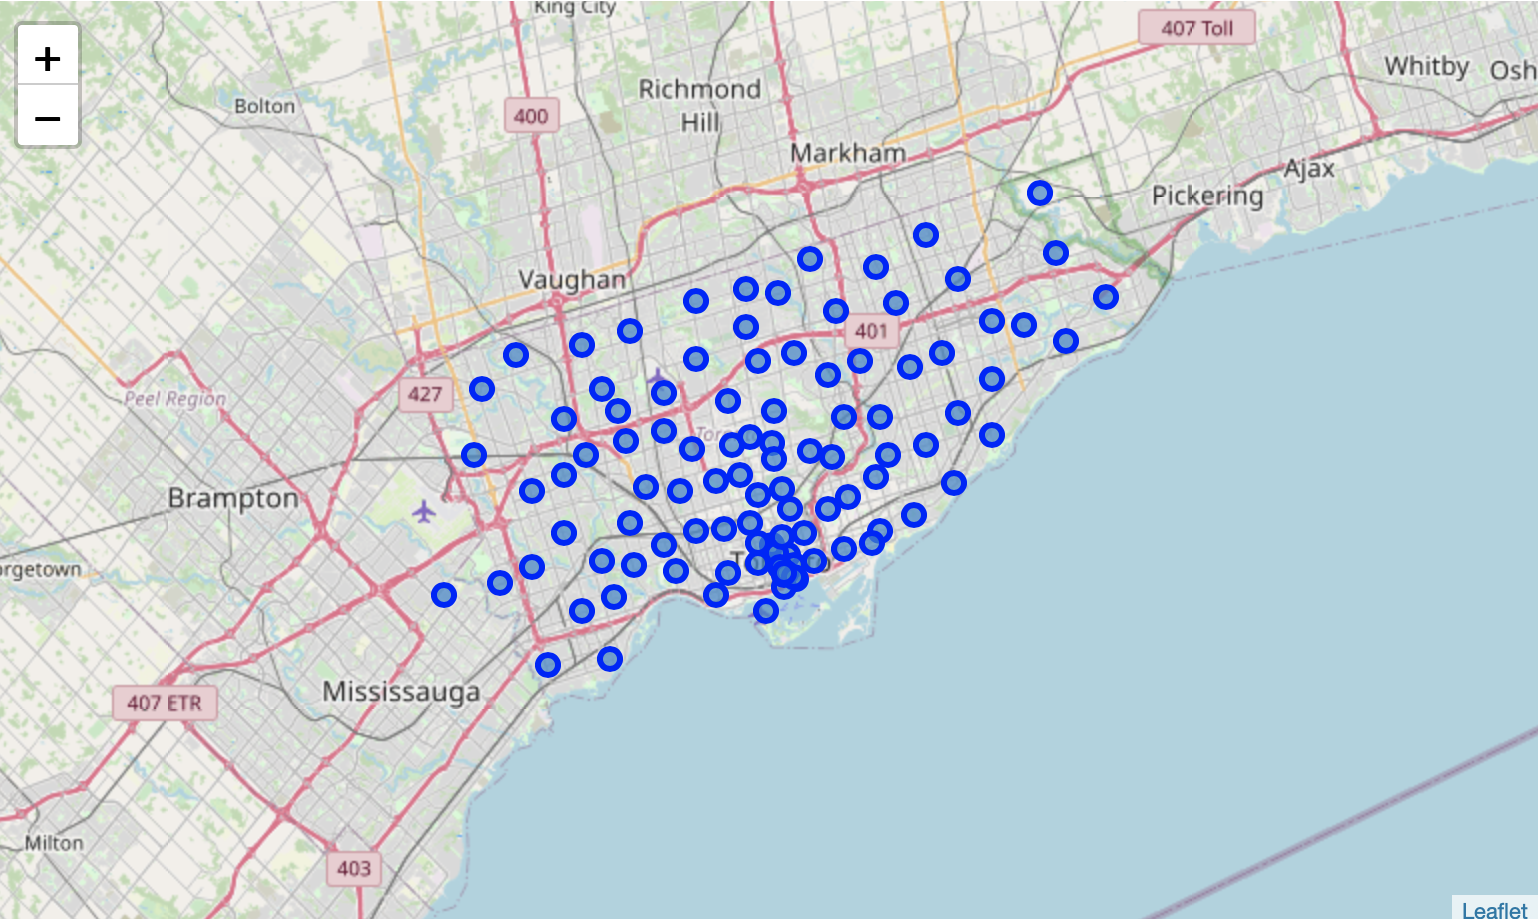
\includegraphics[scale=0.55]{image/1.png}

Then I extract all the venues from FourSquare dataset and group them by venue type as well as neighbors as follows\\
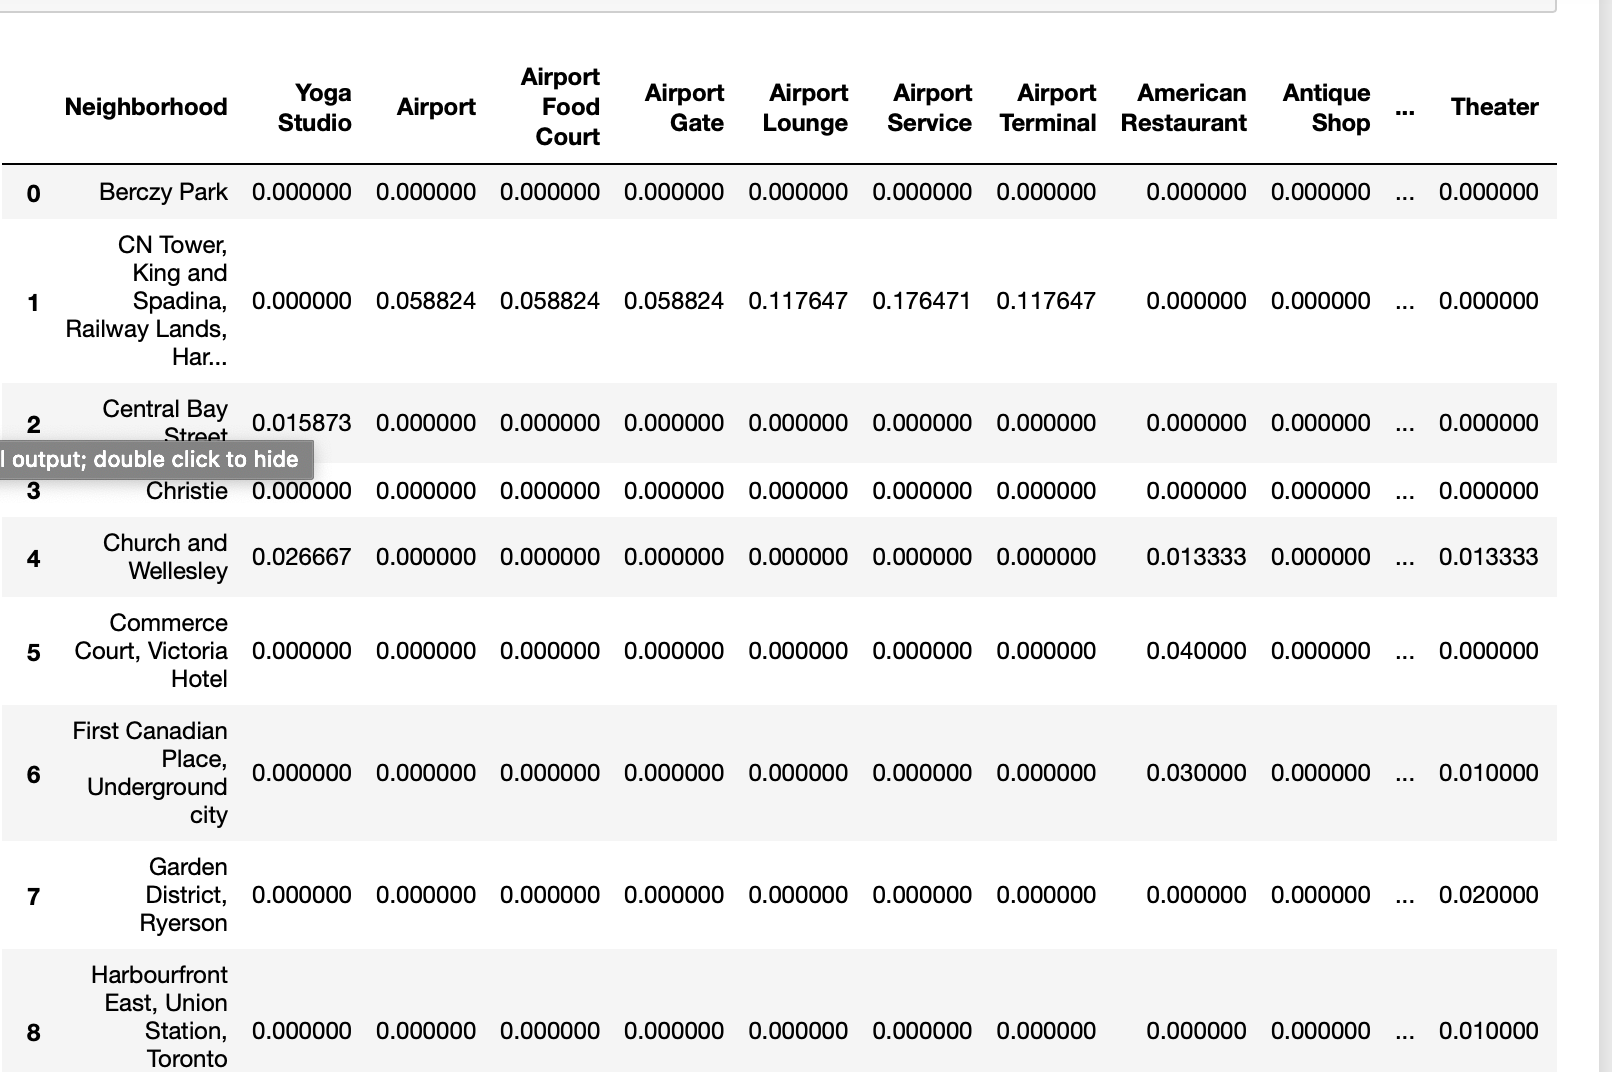
\includegraphics[scale=0.55]{image/2.png}

I also make a rank based on the most popular type of venues within each neighborhood, this is similar to what we did for New York\\
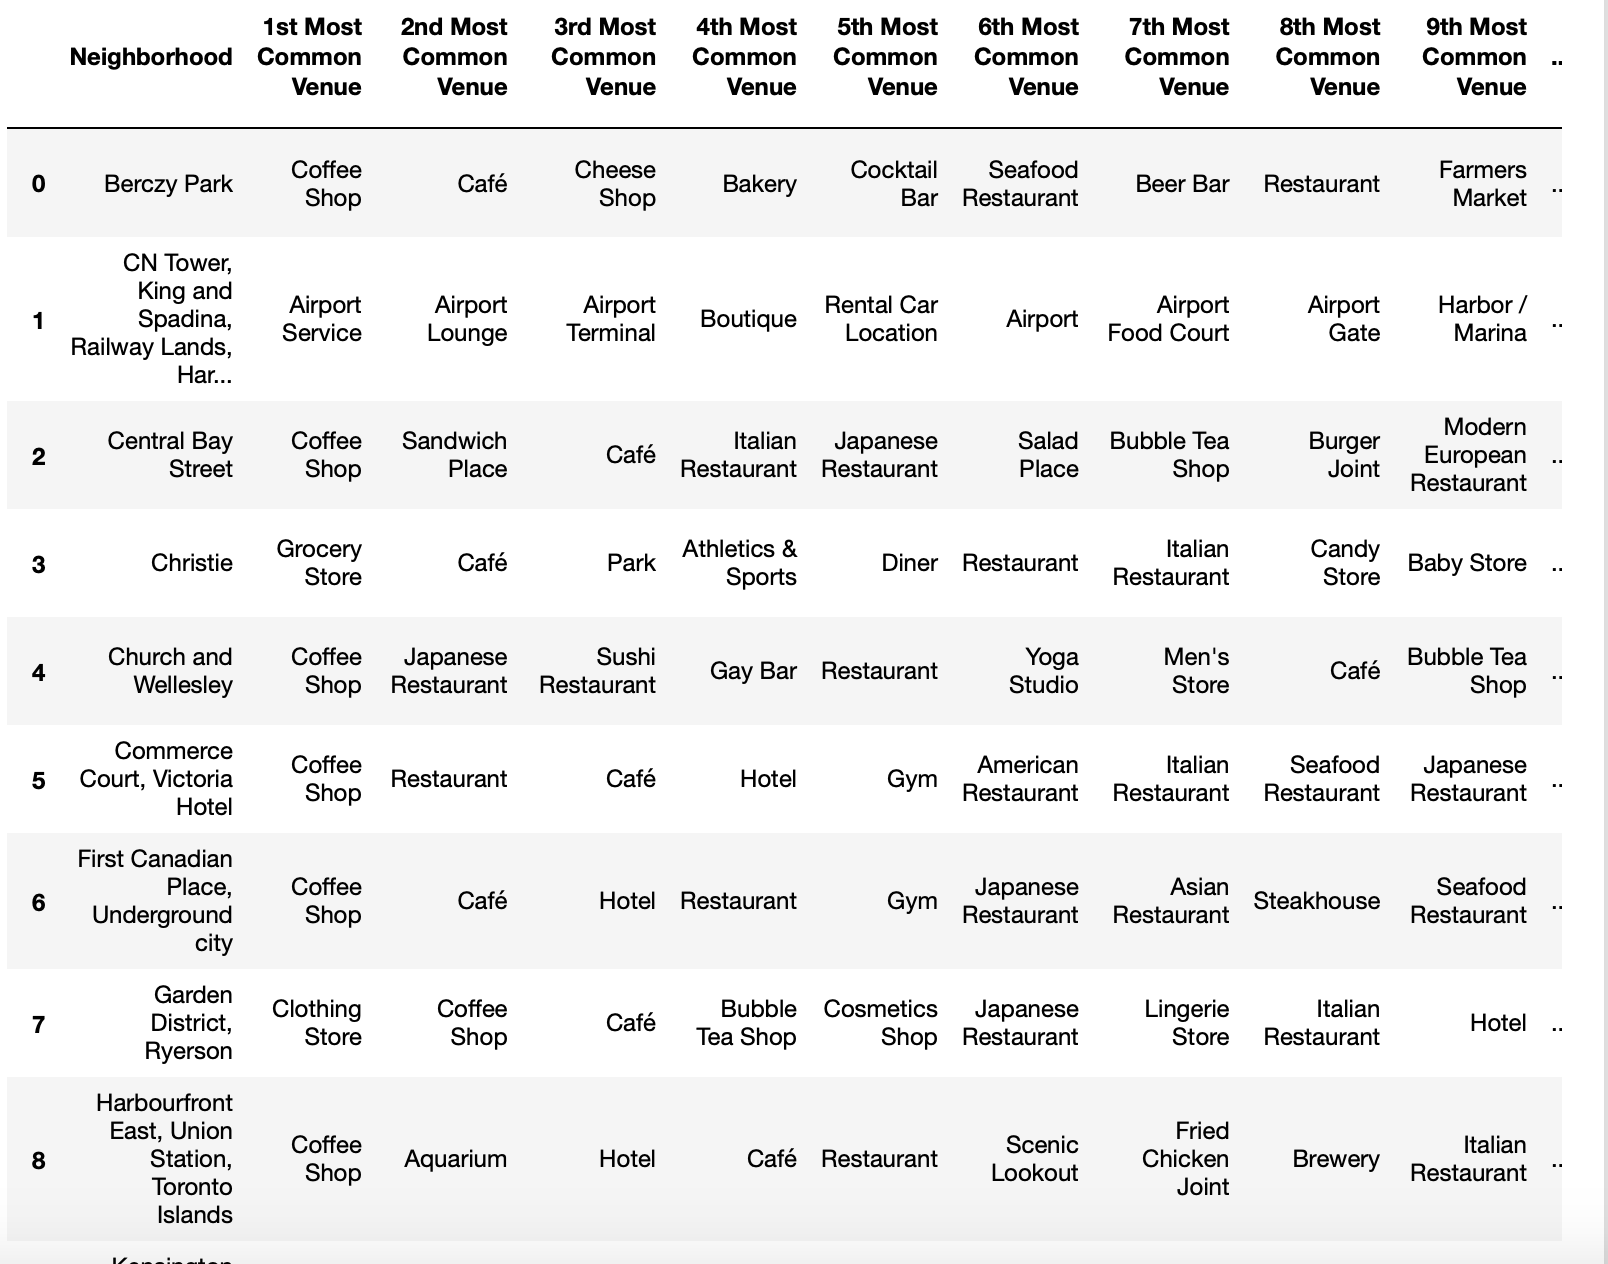
\includegraphics[scale=0.55]{image/3.png}

In the next step, I conduct the main analysis, I first compute the density of restaurants that serve east Asian style food (including Asian Restaurant, Chinese Restaurant, Japanese Restaurant, Korean Restaurant, Sushi Restaurant, Taiwanese Restaurant, Thai Restaurant and Vietnamese Restaurant). The assumption I make is that the east Asian style food are similar so that people who are interested in other types of east Asian style food should have a higher probability to be also interested in Korean style restaurants. Thus I calculate the difference between the density of east Asian style restaurant and Korean restaurant: since the former density is an approximate how many people in this neighborhood might be interested in Korean restaurant and the later density is the current number of Korean restaurant, the difference is a good indicator of how profitable openning a Korean restaurant will be in this neighborhood.

\section{Results and Discussion}
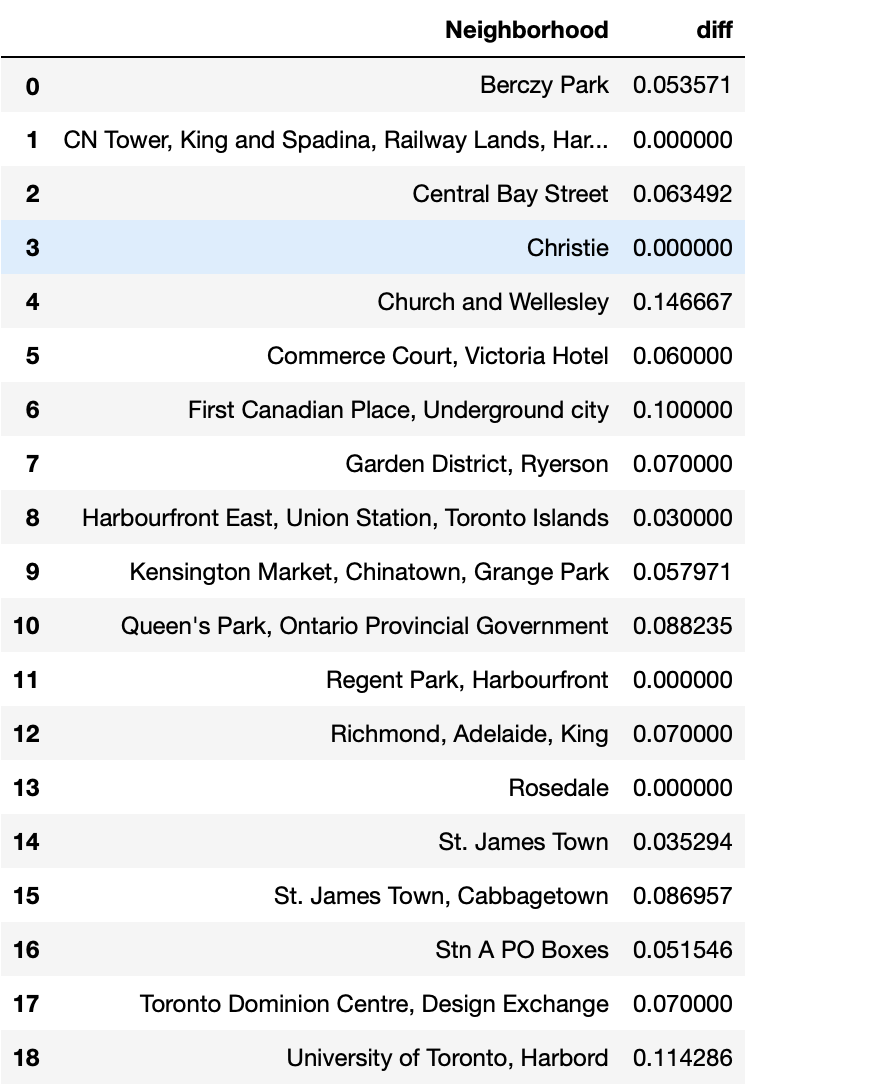
\includegraphics[scale=0.55]{image/4.png}

The difference of density of east Asian restaurants and Korean restaurants is shown in the table above. As we can see, the largest difference appear in neighborhood Church and Wellesley. Since the former density is an approximate how many people in this neighborhood might be interested in Korean restaurant and the later density is the current number of Korean restaurant, the difference is a good indicator of how profitable openning a Korean restaurant will be in this neighborhood, thus I think it's a good idea for Mr. Sammon should open his Korean restaurant in the neighborhood of Church and Wellesley. 

Admittedly, this analysis is pretty naive and preliminary, if more data available, it would be a great idea to analyze the population demographic structure in each neighborhood and also the profitability of existed restaurants to help Mr. Sammon make better decisions.

\section{Conclusion}
Mr. Sammon should open his Korean restaurant in the neighborhood of Church and Wellesley
\section {References}
\bibliographystyle{IEEEtranS}

%\bibliography{capstone}

\end{document}
